\documentclass[tikz]{standalone}
\usepackage{amssymb}
\usepackage{amsfonts}
\usepackage{mathrsfs}
\usepackage{amsthm}
\usepackage{amsmath}
\usepackage{xcolor}
\usepackage{hyperref}
\usepackage{libertinus}
\usepackage{dsfont}
\usepackage{bm}
\usepackage{enumitem}
\usepackage{caption}
\usepackage{subcaption}
\usepackage{tikz}
\usepackage{quiver}

\newcommand{\R}{\mathbb{R}}
\newcommand{\C}{\mathbb{C}}
\newcommand{\N}{\mathbb{N}}
\newcommand{\Z}{\mathbb{Z}}
\newcommand{\Q}{\mathbb{Q}}

% differentials and derivatives
\renewcommand{\d}{\mathrm{d}}
\newcommand{\dd}{\,\d}
\newcommand{\pddf}[2]{\frac{\partial#1}{\partial#2}}
\newcommand{\ddt}{\frac{\d }{\d t}}
\newcommand{\ddtz}{\left.\ddt\right|_{t=0}}

\begin{document}
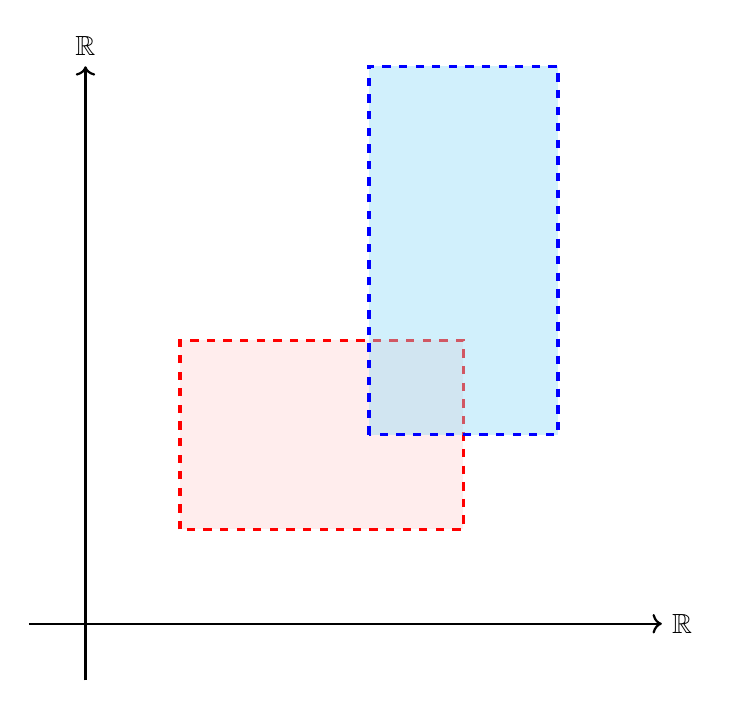
\begin{tikzpicture}[scale=1.2]

    % Axes
    \draw[->, thick] (-0.6,0) -- (6.1,0)
        node[right] {$\mathbb{R}$};
    \draw[->, thick] (0,-0.6) -- (0,5.9)
        node[above] {$\mathbb{R}$};

    % Pink horizontal rectangle
    \fill[pink!70, opacity=0.4] (1.0,1.0) rectangle (4.0,3.0);
    \draw[red, very thick, dashed]
        (1.0,1.0) rectangle (4.0,3.0);

    % Blue vertical rectangle
    \fill[cyan!45, opacity=0.4] (3.0,2.0) rectangle (5.0,5.9);
    \draw[blue, very thick, dashed]
        (3.0,2.0) rectangle (5.0,5.9);

\end{tikzpicture}
\end{document}